
\section {帐号与密码}

    帐号是在网络和多用户操作系统中保存着一种记录,用于记录授权用户的行为。网络帐户由网络管理员创建,用来验证用户和管理与每个用户相关的策略,例如访问权限。账号是数字时代的代表,就是每个人在特定的项目中所代表自己的一些数字等。账号有时可以由中文或英文组成,甚至是一些符号。 在多数场合下会被误写作“帐号”

\subsection {帐号密码的重要性}

    密码是安全基础的核心。如果危及到密码,那个基本的安全机制和模式将遭到严重影响。

    \begin{center}
        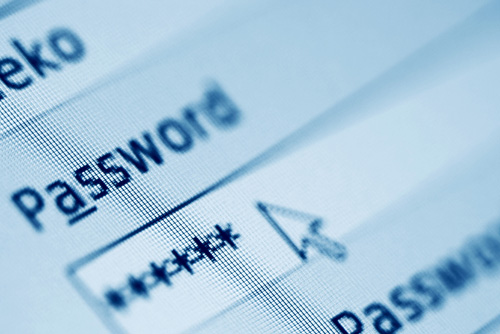
\includegraphics[scale=.6] {password.jpg}
    \end{center}

    一个强固的密码至于要有下列四方面内容的三种:

    \begin{itemize}
        \item 大写字母
        \item 小写字母
        \item 数字
        \item 非字母数字的字符,如标点符号
    \end{itemize}

    强固的密码还要符合下列的规则

    \begin{itemize}
        \item 不使用普通的名字或昵称
        \item 不使用普通的个人信息,如生日日期
        \item 密码里不含有重复的字母或数字
        \item 至少使用八个字符
    \end{itemize}

    从黑客的思想考虑,避免密码容易被猜出或发现(比如不要写到纸条上放到抽屉里)。

    总的来说,个人密码安全需要遵循如下几个简单的要求:对于不同的网络系统使用不同的密码,对于重要的系统使用更为安全的密码。绝对不要所有系统使用同一个密码。对于那些偶尔登录的论坛,可以设置简单的密码;对于重要的信息、电子邮件、网上银行之类,必需设置为复杂的密码。永远也不要把论坛、电子邮箱和银行账户设置成同一个密码。

\subsection {密码分类}

    处于安全考虑,最好将自己的常用密码分类:弱密码、中密码、强密码

    \begin{enumerate}
        \item 弱密码

        最容易记忆的,且默认是可以丢失的密码。

        各类中小网站、论坛、社区、个人网站等使用。

        原因:这些网站的安全性可能都不太好,有些只是将密码MD5一下存储,有些可能还会明文存储密码。黑客很容易从这些网站盗窃用户的密码。

        \item 中密码

        中等强度密码,8个字符以上,有一定抗穷举能力的。

        中等密码主要在国内门户网站、大型网站、门户微博、社交网站等使用,但不要在主要邮箱里使用。门户网站最好绑定手机号码。

        原因:大网站的安全性较好,通常被破解的可能性低,在大网站使用的密码要强度可以稍强。

        需要注意的是,有些门户网站(例如新浪、搜狐等)即提供微博,又提供邮件系统,如果系统默认建立了这些邮箱,那建议不要在任何地方使用这些邮箱,如果要使用邮箱,最好确认该邮箱具有独立密码功能。

        其中有一个例外是腾讯邮箱,腾讯邮箱支持邮箱的单独密码,设置好了以后,用户需要输入QQ密码和邮箱密码两个之后才能使用。

        所有游戏帐号使用单独的密码。

        \item 强密码

        强密码要求至少8个字符以上,不包含用户名、真实姓名或公司名称,不包含完整的单词,包含字母、数字、特殊符号在内。

        强密码主要用于邮箱、网银、支付系统等。

        这类网站是最核心最重要的网站,网银涉及到用户的财产安全,邮箱则可以重置用户所有注册过的网站密码,因此这类网站一定要用强密码,保证其绝对安全性。

        密码穷举对于简单的长度较少的密码非常有效,但是如果网络用户把密码设的较长一些而且没有明显规律特征(如用一些特殊字符和数字字母组合),那么穷举破解工具的破解过程就变得非常困难,破解者往往会对长时间的穷举失去耐性。通常认为,密码长度应该大于8位,密码中最好包含字母数字和符号,不要使用纯数字的密码,不要使用常用英文单词的组合,不要使用自己的姓名做密码,不要使用生日做密码。
    \end{enumerate}
